As shown in the UX Diagram below, the user must first select if he is a \textit{Run Organizer} or a \textit{Normal User}, then he can proceed in choosing wheather he wants to login or register. \\
The \textit{Login} and \textit{Registration} flow are similar, being associated with similar procedures.
The only difference is that, due to the fact that a SmartWatch is required for the \textit{Normal User} to use the app, the presence of it is checked during \textit{Login} and \textit{Registration}.
\\
If the procedures mentioned before are successful the user lands on the \textit{Main Screen}, on which a Navigation Drawer presents him the \textit{Navigation Options}.\\ \\
\noindent If the User is a \textit{Run Organizer} the options are the following: 
\begin{itemize}
    \item View All Runs
    \item Organize a Run
\end{itemize}
\vspace{0.5cm}
If the User is a \textit{Normal User} the options are the following: 
\begin{itemize}
    \item Health Graph
    \item All Runs Available
    \item AutomatedSOS
\end{itemize}

\vspace{0.5cm}
\noindent If the \textit{Run Organizer} selects the \textit{View All Runs} option he is presented with a screen in which all run organized by him are present. Tapping on a run results in a screen with all the information concerning it shown.
If the \textit{Run Organizer} selects the \textit{Organize a run} option he is presented with the \textit{Run Organization Form} screen which will be followed by, after submission, the \textit{Run Info} screen.

\vspace{0.5cm}
\noindent The \textit{Normal User} has the possibility to: 
\begin{itemize}
    \item View the \textit{Health Graph} screen, by which, tapping on a graph, results in more information concerning the selected health parameters being shown.
    \item See \textit{All Runs Available}, by which, tapping on a run, results in more informations on the run being show.
    \item Subscribe to \textit{AutomatedSOS}.
\end{itemize}

\begin{figure}
        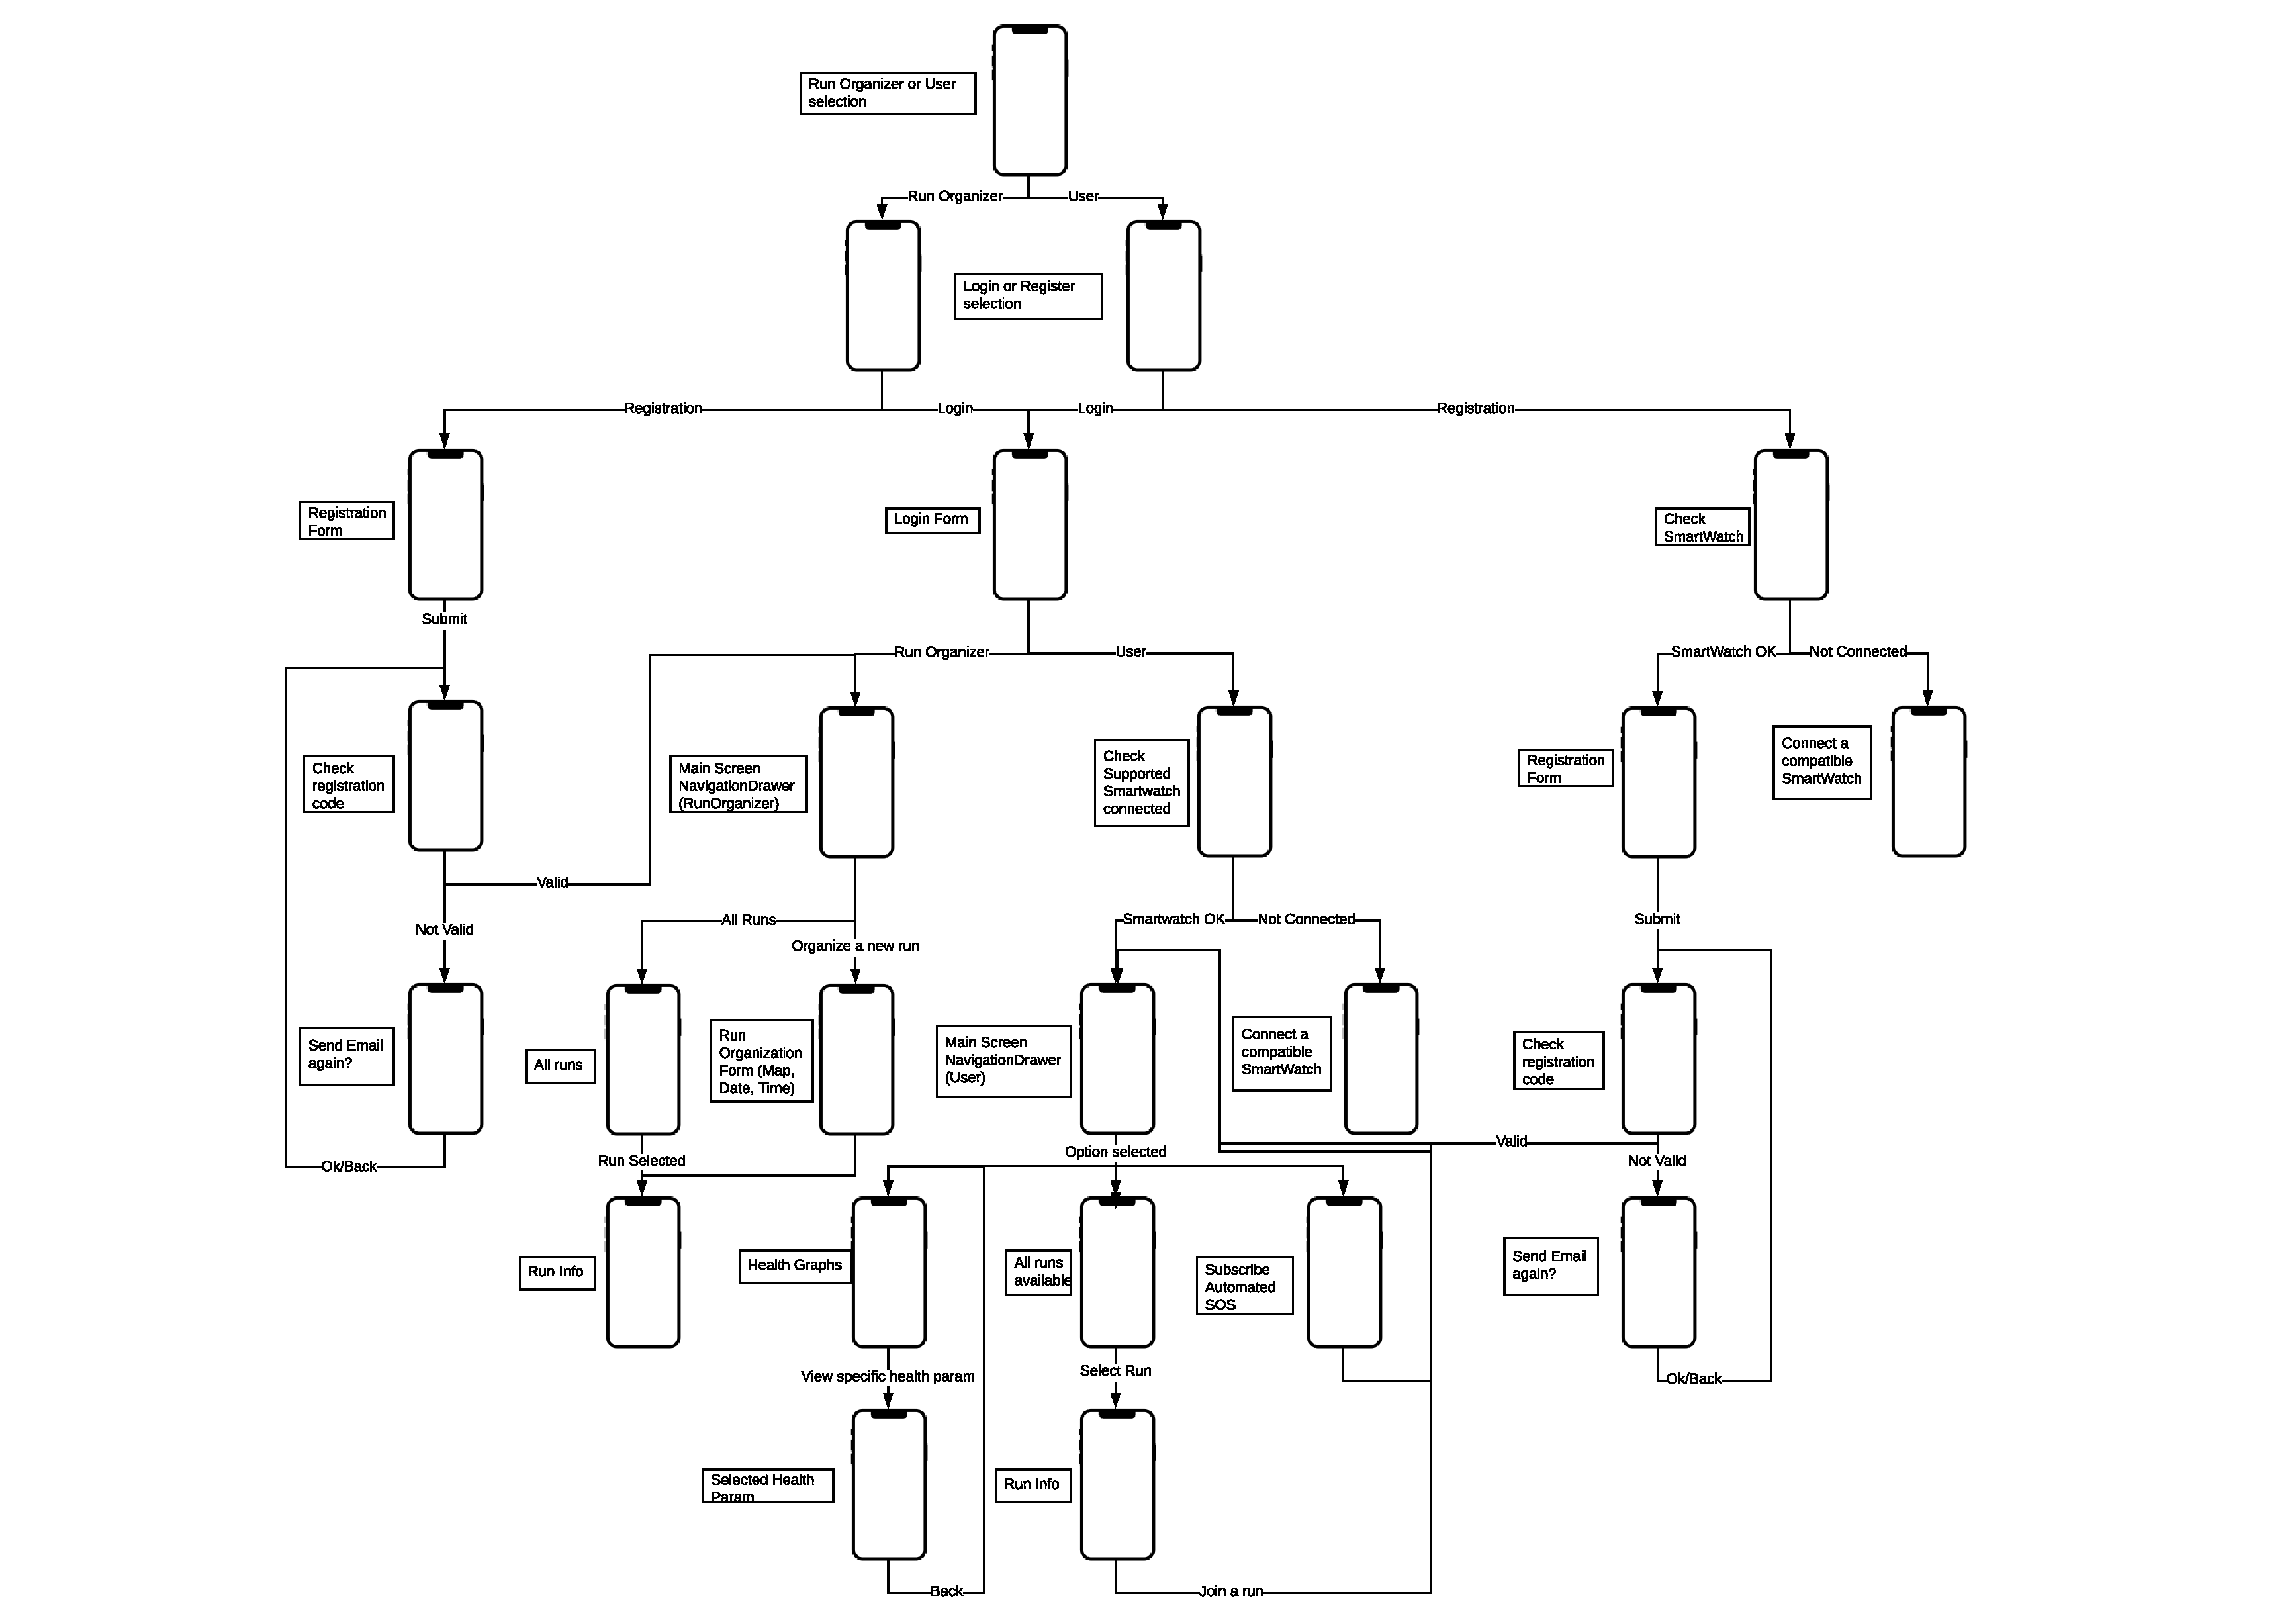
\includegraphics[width=\textwidth,height=\textheight,keepaspectratio]{assets/flowCharts/UXDiagramMobile.pdf}
    \caption{UX Diagram for Website}
    \label{fig:UXDiagram}
\end{figure}







\begin{figure}
        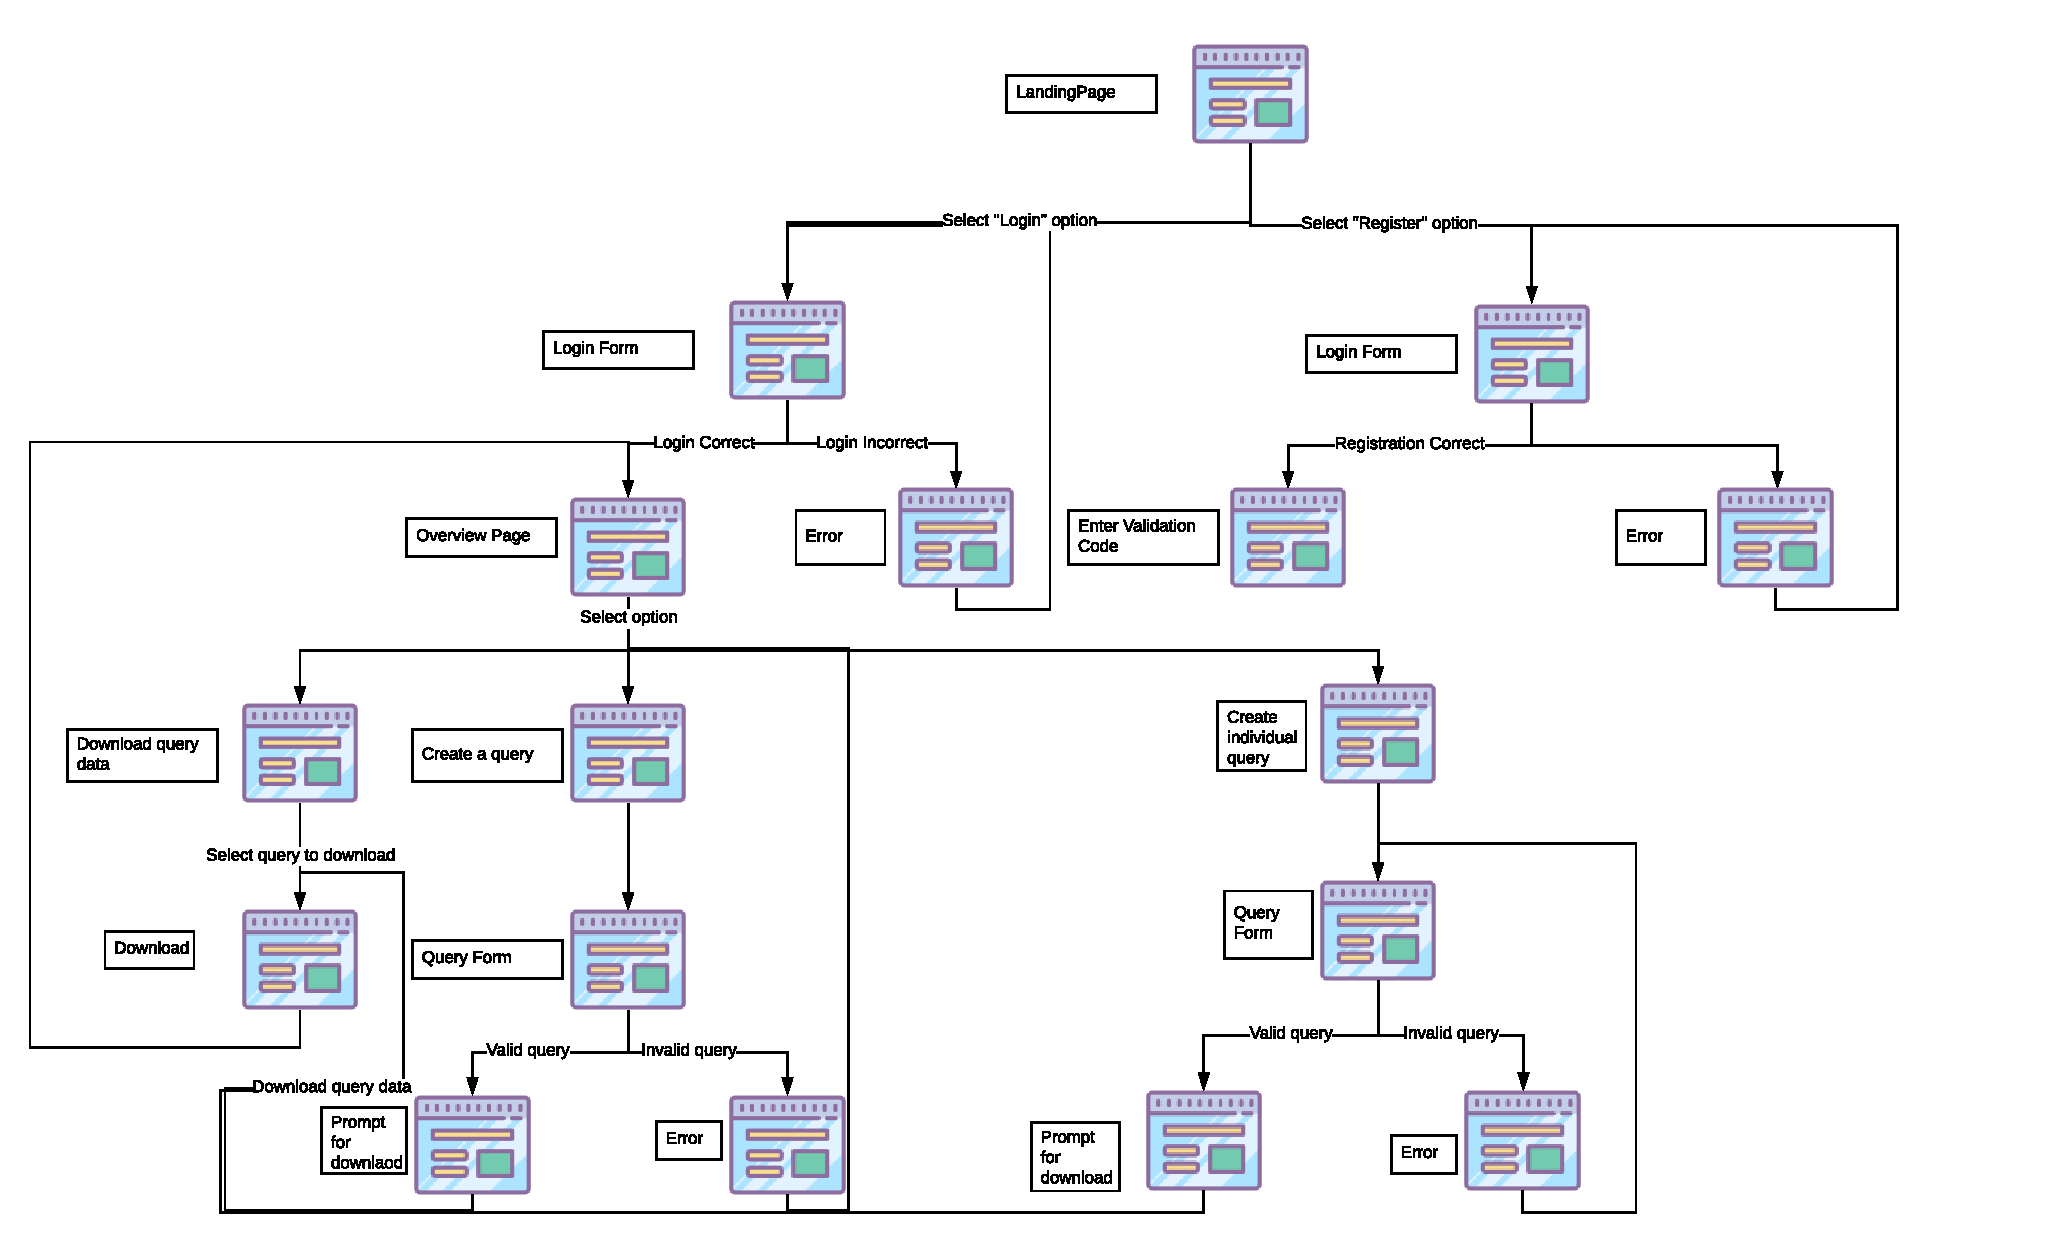
\includegraphics[width=\textwidth,height=\textheight,keepaspectratio]{assets/flowCharts/UXDiagramWebsite.pdf}
    \caption{UX Diagram for Mobile App}
    \label{fig:uxWebsite}
\end{figure}
